%!TEX ROOT=main.tex
\chapter{Implementace}


\section{Pneumatická část}

Pneumatická čast systému je část ve které probíhá měření měření hemodynamických parametrů srdce pacienta. Je to jediná čast systému, která přichází v přímý kontakt s pacientem.
\begin{figure}[H]
    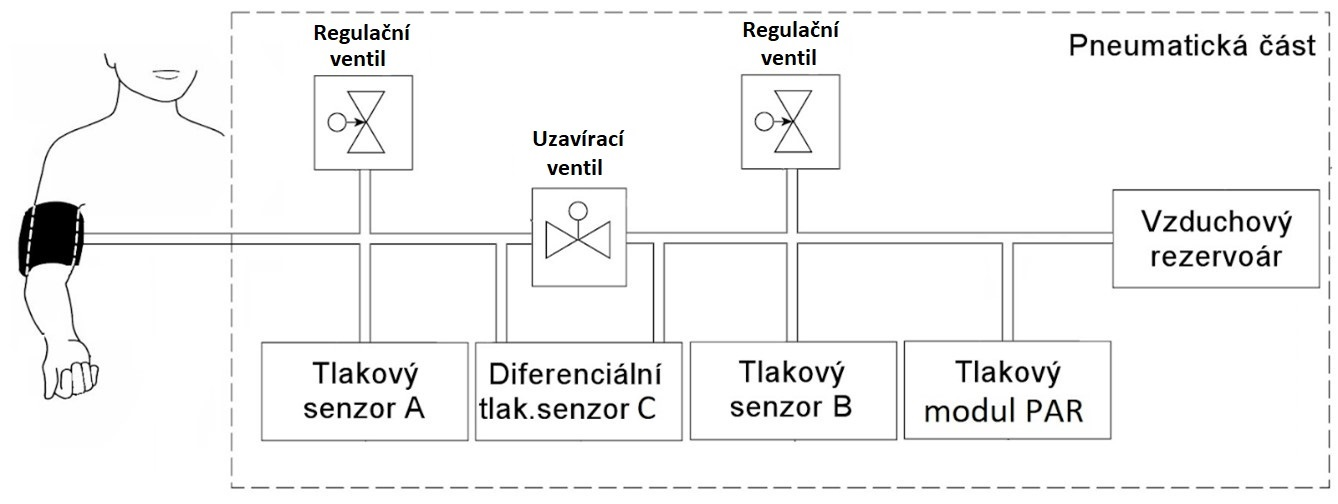
\includegraphics[width=1\linewidth]{pictures/blokove_schema_pneu.jpg}
    \caption{Blokové schéma pneumatického systému}
    \label{fig:pneu_block}
\end{figure}

\subsection{Měření těsnosti penumatické časti}
Pneumatická čast musí být co nejlépe těsná, aby po dobu terapie byl co nejmešní úbytek tlaku v systému.
\par
Test těsnosti probíhal pomocí přístroje FLUKE Biomedical BP pump 2, který natlakoval pneumatickou část na hodnotu 200 mmHg a následně sledoval úbytek tlaku v systému po dobu 60 s.
Měření bylo opakováno 10 krát po sobě.

\begin{table}
    \label{tab:pressure_test_pneu}
    \caption{Test těstnosti pneumatického systému}
    \begin{tabular}{ccc}
        \toprule
        Měření & Těsnost & Jednotky           \\ \midrule
        1      & 0.9     &                    \\
        2      & 0.8     &                    \\
        3      & 1.1     &                    \\
        4      & 1.0     &                    \\
        5      & 0.9     & $\frac{mmHg}{min}$ \\
        6      & 0.9     &                    \\
        7      & 1.1     &                    \\
        8      & 0.9     &                    \\
        9      & 0.8     &                    \\
        10     & 1.0     &                    \\
        \bottomrule
    \end{tabular}
\end{table}

\subsection{Zkreslení signálu pneumatickým systémem}
Přenosová funkce systému byla identifikována měřením impulzní odezvy systému. Systém byl natlakovám na průměrnou hodnotu suprasystolického tlaku 230 mmHg a poté
byl aplikován jednotkový impuls pomocí mechanického kyvadla.
\begin{figure}[H]
    \label{fig:mech_kyvadlo}
    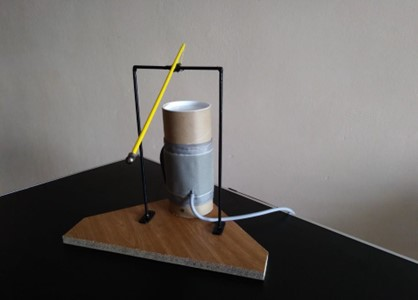
\includegraphics[width=1\textwidth]{pictures/mech_kyvadlo.jpg}
    \caption{Mechaniké kyvadlo pro vytvoření jednotkového impulsu na pneumatický systém.}
\end{figure}
\begin{figure}[H]
    \label{fig:pneu_impulse_response}
    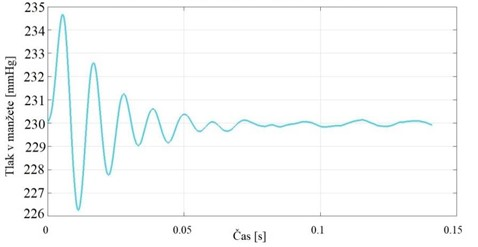
\includegraphics[width=1\textwidth]{pictures/pneu_impulse.jpg}
    \caption{Odezva pneumatického systému na jednotkový impuls.}
\end{figure}
Z naměřené hodnoty impulzní odezvy byly vypočteny parametry vlastní frekvence $f_0 \ [Hz]$ a poměrného útlumu $\xi \ [-]$. Pomocí těchto parametrů, za předpokladu, že se jedná o dynamický systém druhého řádu, bylo možné vypočítat přenosovou funkci systému.
\begin{figure}[H]
    \caption{Odezva pneumatického systému na jednotkový impuls.}
    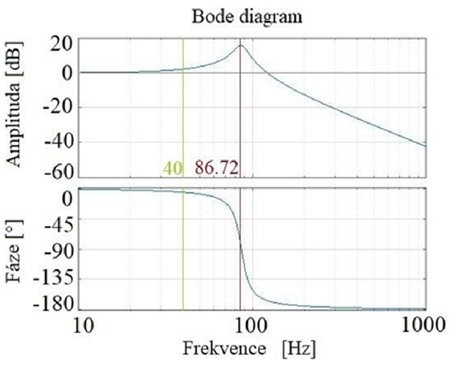
\includegraphics[width=1\textwidth]{pictures/freq_char_pneu.png}
    \label{fig:pneu_freq_char}
\end{figure}
Při měření srdečních frekvencí např. 120 tepů/min tj. 2 Hz, odpovídá 20. harmonická složka tepu frekvenci $f = 40 \ Hz$. Podle obrázku \ref{fig:pneu_freq_char} srdeční frekvence je amplituda zkreslena o +2 dB a fáze signálu o $^\circ 5$, což jsou akceptovatelné hodnoty.
